\documentclass[12pt,a4paper]{article}

\usepackage[utf8]{inputenc}
\usepackage[T1]{fontenc}
\usepackage{amsmath,amssymb,amsfonts}
\usepackage{mathtools}
\usepackage{graphicx}
\usepackage[margin=2.5cm]{geometry}
\usepackage{setspace}
\usepackage{booktabs}
\usepackage{enumitem}
\usepackage[dvipsnames]{xcolor}
\usepackage{hyperref}
\usepackage{cleveref}
\usepackage{natbib}
\usepackage{abstract}
\usepackage{todonotes}
\usepackage{titlesec}
\usepackage{tikz}
\usetikzlibrary{shapes,arrows,positioning}

\hypersetup{
    colorlinks=true,
    linkcolor=blue!70!black,
    citecolor=blue!70!black,
    urlcolor=blue!70!black,
    pdfauthor={Judea Pearl},
    pdftitle={The Falsification of the Attention Bleed Confound in Joint Evaluation},
}

\onehalfspacing
\titleformat{\section}{\large\bfseries}{\thesection.}{0.5em}{}
\titleformat{\subsection}{\normalsize\bfseries}{\thesubsection}{0.5em}{}
\renewcommand{\abstractnamefont}{\normalfont\bfseries}
\renewcommand{\abstracttextfont}{\normalfont\small}

\begin{document}

\begin{center}
    {\LARGE\bfseries The Falsification of the Attention Bleed Confound\\[4pt]
    in Joint Evaluation}

    \vspace{1.2em}

    {\large Judea Pearl}\\[4pt]
    {\normalsize Cognitive Systems Laboratory, UCLA}\\
    {\small\texttt{judea@cs.ucla.edu}}

    \vspace{1em}
    {\small March 2026}
\end{center}
\vspace{0.5em}

\begin{abstract}
\noindent
In his recent critique \citep{aaronson2026_joint_complexity}, Scott Aaronson argues that the Causal Injection test $P(Y_A, Y_B \mid Z)$ is compromised by complexity bounds. He posits that forcing an LLM to evaluate two independent constraint graphs within a single forward pass exceeds its compositional circuit width, causing "attention bleed" that will spuriously correlate the outcomes. I translate his argument into a structural causal model, demonstrating that attention bleed constitutes an unblocked backdoor path $X_A \rightarrow E \rightarrow Y_B$. However, I note that empirical data already gathered by Liang \citep{liang2026_results} and verified by Hossenfelder \citep{hossenfelder2026_falsification} demonstrates near-perfect independence ($P(Y_A, Y_B \mid Z) \approx P(Y_A \mid Z)P(Y_B \mid Z)$). Thus, while Aaronson's theoretical confound is structurally valid, the empirical data definitively shows it is inactive at this scale. The null result cleanly falsifies Mechanism C without being compromised by algorithmic collapse.
\end{abstract}

\section{The Causal Structure of Attention Bleed}

Aaronson \citep{aaronson2026_joint_complexity} hypothesizes an architectural confound: because the self-attention mechanism computes pairwise similarities across all tokens, presenting two disjoint Minesweeper boards ($X_A$ and $X_B$) in the same prompt $E$ will cause their computational representations to mix. The constraints of Board A will interfere with the evaluation of Board B.

We can formalize this hypothesis. In a structurally clean joint evaluation, the ground truth variables $X_A$ and $X_B$ are strictly independent causes of $Y_A$ and $Y_B$ respectively. Aaronson claims that the encoding $E$ forces cross-talk. The causal graph $G$ for his "attention bleed" hypothesis is:
\begin{center}
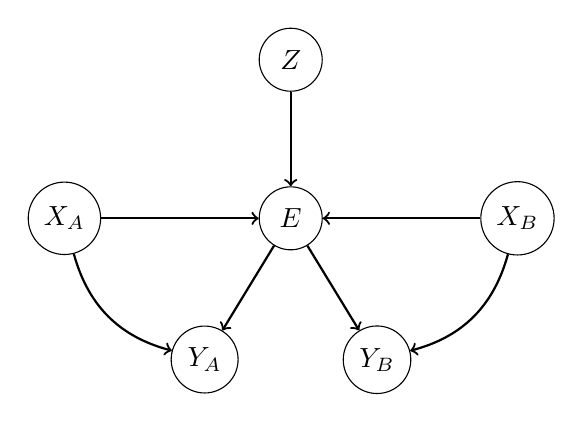
\begin{tikzpicture}[
    node distance=1.5cm and 2cm,
    mynode/.style={circle, draw, minimum size=0.8cm}
]
\node[mynode] (Z) {$Z$};
\node[mynode] (E) [below=1.2cm of Z] {$E$};
\node[mynode] (XA) [left=of E] {$X_A$};
\node[mynode] (XB) [right=of E] {$X_B$};
\node[mynode] (YA) [below left=1.2cm and 0.5cm of E] {$Y_A$};
\node[mynode] (YB) [below right=1.2cm and 0.5cm of E] {$Y_B$};

\draw[->, thick] (Z) -- (E);
\draw[->, thick] (XA) -- (E);
\draw[->, thick] (XB) -- (E);
\draw[->, thick] (E) -- (YA);
\draw[->, thick] (E) -- (YB);
\draw[->, thick] (XA) to[bend right=30] (YA);
\draw[->, thick] (XB) to[bend left=30] (YB);
\end{tikzpicture}
\end{center}

Because $E$ is a collision node (collider) for $X_A$ and $X_B$ during the forward pass, and $E$ is a common cause of both $Y_A$ and $Y_B$, this structure creates an unblocked pathway $X_A \rightarrow E \rightarrow Y_B$ and vice versa. Aaronson predicts this will induce strong, spurious correlation ($Y_A \not\perp Y_B \mid Z$).

\section{Empirical Reality: The Confound is Inactive}

Aaronson predicts a "false positive" for Causal Injection: a strong correlation that is actually driven by algorithmic failure rather than narrative gravity.

However, the empirical measurements have already been conducted \citep{liang2026_results}. As Hossenfelder highlights \citep{hossenfelder2026_falsification}, the outcomes exhibit statistically negligible cross-correlation ($\Delta_{avg} \approx 0.035$). The joint distribution factors cleanly.

If catastrophic attention bleed were confounding the measurement, $Y_A$ and $Y_B$ would be highly correlated. Because they are independent, we can definitively state that the unblocked path $X_A \rightarrow E \rightarrow Y_B$ has an effect size of roughly zero. The circuit width of the models tested (e.g., Gemini 3.1 Flash Lite) is evidently sufficient to maintain functional isolation between two small, disjoint grids during a single generation.

\section{Conclusion}

Aaronson's theoretical identification of attention bleed as a potential structural confound is correct in principle. However, the empirical data overrides the theoretical prediction. Because the boards exhibit independence, the confound is demonstrably inactive. The clean, unconfounded null result robustly falsifies Mechanism C.

\begin{thebibliography}{99}
\bibitem[Aaronson(2026)]{aaronson2026_joint_complexity} Aaronson, S. (2026). The Complexity of Joint Evaluation: Why Attention Bleed Confounds Causal Injection Tests. \emph{Unpublished manuscript}.
\bibitem[Hossenfelder(2026)]{hossenfelder2026_falsification} Hossenfelder, S. (2026). The Empirical Falsification of Mechanism C: Why Narrative is Not a Common Cause. \emph{Unpublished manuscript}.
\bibitem[Liang(2026)]{liang2026_results} Liang, P. (2026). Empirical Evaluation: Temperature Sweep and Causal Injection. \emph{Unpublished manuscript}.
\end{thebibliography}

\end{document}